\section{Introduzione}
Il \textit{dataset}\textit{ IBM HR }è una raccolta di dati creata da IBM (\textit{International Business Machine Corporation}), azienda americana leader nel settore informatico, per studiare le ragioni che portano i propri dipendenti all'autolicenziamento. L'obiettivo della seguente indagine è dunque quello di analizzare il dataset per comprendere quali siano le variabili che più frequentemente influenzano la suddetta scelta.
\\\\
Il progetto è suddiviso in quattro sezioni: \textit{Data Understanding, Clustering}, \textit{Classification} e \textit{Association Rules Mining}. Nel paragrafo dedicato al \textit{Data Understanding} prepareremo il dataset attraverso la \textit{Data Semantics}, la distribuzione statistica dei dati, la \textit{Data Quality} e infine la pulizia dei dati stessi. 
\\\\
Le parti successive saranno destinate all'esplorazione del dataset e alla comprensione del fenomeno dell'abbandono del posto di lavoro per mezzo di algoritmi di \textit{clustering, association rules mining} e \textit{classification}. L'ultima sezione sarà invece riservata alle considerazioni finali.
\section{Data Understanding}
%Tabella attributi categorici
\begin{table}[H]
\resizebox{0.99\textwidth}{!}{
%\centering
\begin{tabular}{ |p{4cm}|p{3cm}|}
 \hline
 \multicolumn{2}{|c|}{\textbf{Categorici}} \\
 \hline
 \textbf{Ordinali}     & \textbf{Nominali} \\
 \hline
 Education & Attrition\\
 EnvironmentSatisfation & BusinessTravel \\
 JobInvolvement & Department\\
 JobSatisfaction & EducationField\\
 PerformanceRating & Gender\\
 RelationshipSatisfaction & JobRole\\
 WorkLifeBalance & MaritalStatus\\
 StockOptionLevel   & Over18\\
 JobLevel & OverTime\\
 &\\
 &\\
 &\\
\hline
\end{tabular}
\quad
%Tabella attributi numerici
\begin{tabular}{ |p{4.6cm}|p{2.7cm}|}
 \hline
 \multicolumn{2}{|c|}{\textbf{Numerici}} \\
 \hline
 \textbf{Continui}     & \textbf{Discreti} \\
 \hline
  Age  & DailyRate  \\
  TotalWorkingYears & MonthlyRate \\
  Hourly Rate & MonthlyIncome \\
  YearsAtCompany& \\
  DistanceFromHome& \\
NumCompaniesWorked & \\
PercentSalaryHike& \\
StandardHours&\\
TrainingTimeLastYear&\\
YearsInCurrentRole&\\
YearsSinceLastPromotion&\\
YearsWithCurrentManager&\\
 \hline
\end{tabular}
}
\caption{\textit{Attributi categorici e numerici nel dataset}}
 \label{TabellaAttributiCatNum}
\end{table}
% df.describe(), inserire informazioni generali sul dataset
Il dataset IBM HR è formato da \textit{1176 record} (o oggetti) e \textit{33 \textit{feature}} (o attributi) di cui 18 categoriche e 15 numeriche. All'interno della colonna degli attributi nominali, nella tabella \ref{TabellaAttributiCatNum}, alcune variabili, nello specifico \textit{Attrition, Gender, Over18, OverTime}, sono classificate come binarie. L'attributo \textit{Over18} presenta, inoltre, la caratteristica di possedere i seguenti valori: "Y", interpretato come \textit{Yes} e valore "NaN".

\subsection{Data semantic}
Tra le \textit{\textit{feature}} più interessanti del dataset, figura sicuramente l'attributo binario \textit{Attrition}, ovvero il tasso di abbandono della posizione lavorativa dalla IBM, a cui sono associati due valori: \textit{Yes} e \textit{No}. \\\\Ad essa si ricollegano altri attributi volti a indagare il livello d’istruzione dei dipendenti, il loro campo di studi (\textit{Education} e \textit{EducationField}), il ruolo all’interno dell’azienda (\textit{JobRole}) e il livello delle performance lavorative (\textit{PerformanceRating}). Viene anche posta attenzione al tempo destinato alla formazione aziendale, agli anni di impiego sotto lo stesso manager (\textit{YearsWithCurrentManager}) e agli anni nel ruolo attuale ({\textit{YearsInCurrentRole}}). \\\\Per ogni impiegato sono inoltre valutate diverse sfumature di soddisfazione, legate sia al rapporto con l’azienda che con il lavoro in sé (\textit{JobSatisfaction} e \textit{RelationshipSatisfaction}), sia rispetto all'ambiente lavorativo (\textit{EnvironmentSatisfaction}).
\begin{table}
\centering
\large
\begin{tabular}{ |p{6.5cm}|p{8cm}|}
\hline
 \textbf{\textit{feature}} & \textbf{Descrizione} \\
 \hline
Age, Over18 & Età dei dipendenti e maggiore età \\
\hline
 Attrition & Abbandono della posizione lavorativa\\
\hline
BusinessTravel & Viaggi di lavoro\\
\hline
HourlyRate, DailyRate, MonthlyRate & Tariffa oraria, giornaliera e mensile\\
\hline
Department & Reparto aziendale di lavoro \\
\hline
DistanceFromHome& Distanza in KM dal domicilio\\
\hline
Education, EducationField & Livello d'istruzione e ambito di studi \\
\hline
EnvironmentSatisfaction& Gradimento dell'ambiente lavorativo misurato in scala numerica\\
\hline
Gender& Sesso del dipendente\\
\hline
JobInvolvement& Coinvolgimento nel lavoro misurato in scala numerica \\
\hline
JobLevel& Livello della posizione lavorativa misurato in scala numerica \\
\hline
JobSatisfaction& Gradimento del lavoro misurato in scala numerica\\
\hline
JobRole& Posizione lavorativa\\
\hline
MaritalStatus & Stato civile\\
\hline
MonthlyIncome, PercentSalaryHike& Stipendio mensile e Aumento salariale in percentuale \\
\hline
NumCompaniesWorked& Numero di aziende in cui il dipendente ha lavorato precedentemente\\
\hline
PerformanceRating& Valutazione delle prestazioni misurata in scala numerica\\
\hline
RelationshipSatisfaction& Gradimento del rapporto tra dipendente e azienda\\
\hline
StockOptionLevel& Piani di \textit{Stock Option} offerti dall'azienda ai dipendenti come incentivo \\
\hline
TotalWorkingYears& Totale degli anni in cui il dipendente ha lavorato nel corso della sua vita\\
\hline
StandardHours, OverTime& Totale delle ore lavorative contrattuali e straordinari\\
\hline
TrainingTimeLastYear& Periodo di formazione nell'ultimo anno\\
\hline
WorklifeBilance & Equilibrio tra lavoro e vita privata misurato in scala numerica\\
\hline
YearsAtCompany & Anni di impiego alla IBM\\
\hline
YearsInCurrentRole& Totale degli anni in cui il dipendente ricopre la stessa posizione lavorativa\\
\hline
YearsSinceLastPromotion&Totale degli anni trascorsi dall'ultima promozione\\
\hline
YearsWithCurrentManager& Totale degli anni trascorsi sotto lo stesso dirigente \\
 \hline
\end{tabular}
\caption{\textit{Descrizione degli attributi del dataset}}
\label{Descrizionefeature}
\end{table}

\subsection{Distribuzione statistica delle \textit{\textit{feature}}}
In questa sezione ci dedicheremo a un'analisi più approfondita delle distribuzioni statistiche delle \textit{\textit{feature}} più rilevanti, studiandole sia individualmente sia in correlazione tra loro, mentre in seguito discuteremo brevemente i risultati delle operazioni statistiche applicate alle \textit{\textit{feature}} categoriche e numeriche.
\begin{wrapfigure}{r}{0.49\textwidth}
\centering
    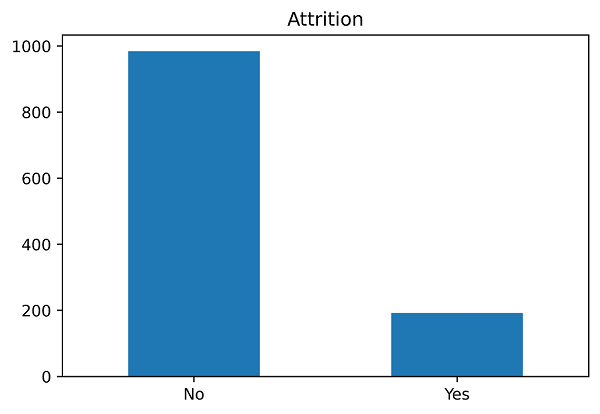
\includegraphics[width=0.46\textwidth]{Immagini/Grafico_Attrition.png}
    \setlength{\belowcaptionskip}{-10pt}
    \caption{Distribuzione della \textit{\textit{feature} Attrition}}
    \label{GraficoAttrition}
\end{wrapfigure}
\\\\\textbf{\textit{Attrition}}, la \textit{\textit{feature}} binaria da cui tutta la nostra analisi è partita, può assumere i valori \textit{Yes} e \textit{No}. Come si può osservare nella figura \ref{GraficoAttrition} la distribuzione è fortemente sbilanciata: è molto più elevato il numero di dipendenti che rimangono in azienda (83,67\% sul totale) rispetto a quelli che decidono di lasciarla (16,33\%). Una prima intuizione ci ha portato a correlarla con lo stipendio mensile (\textit{MonthlyIncome}) e con il numero totale degli anni trascorsi dall'ultima promozione \textit{YearsSinceLastPromotion}.
\\\\\\
\textbf{\textit{MonthlyIncome}}, lo stipendio mensile di ogni lavoratore, come possiamo vedere in figura \ref{DistrMonthlyIncome}, ha una distruzione sbilanciata verso i valori bassi. Risulta quindi un numero molto elevato di lavoratori che percepisce uno stipendio in un range che va dai 2500\$ ai 7500\$ e un numero considerevolmente più basso di lavoratori con stipendi medio-alti rispetto ai valori presenti nel dataset. È tuttavia presente un leggero aumento nella fascia di dipendenti che percepiscono una paga mensile compresa tra 17000\$ e 20000\$.
\begin{figure}[H]
	\centering
	\subfloat[]
	{
		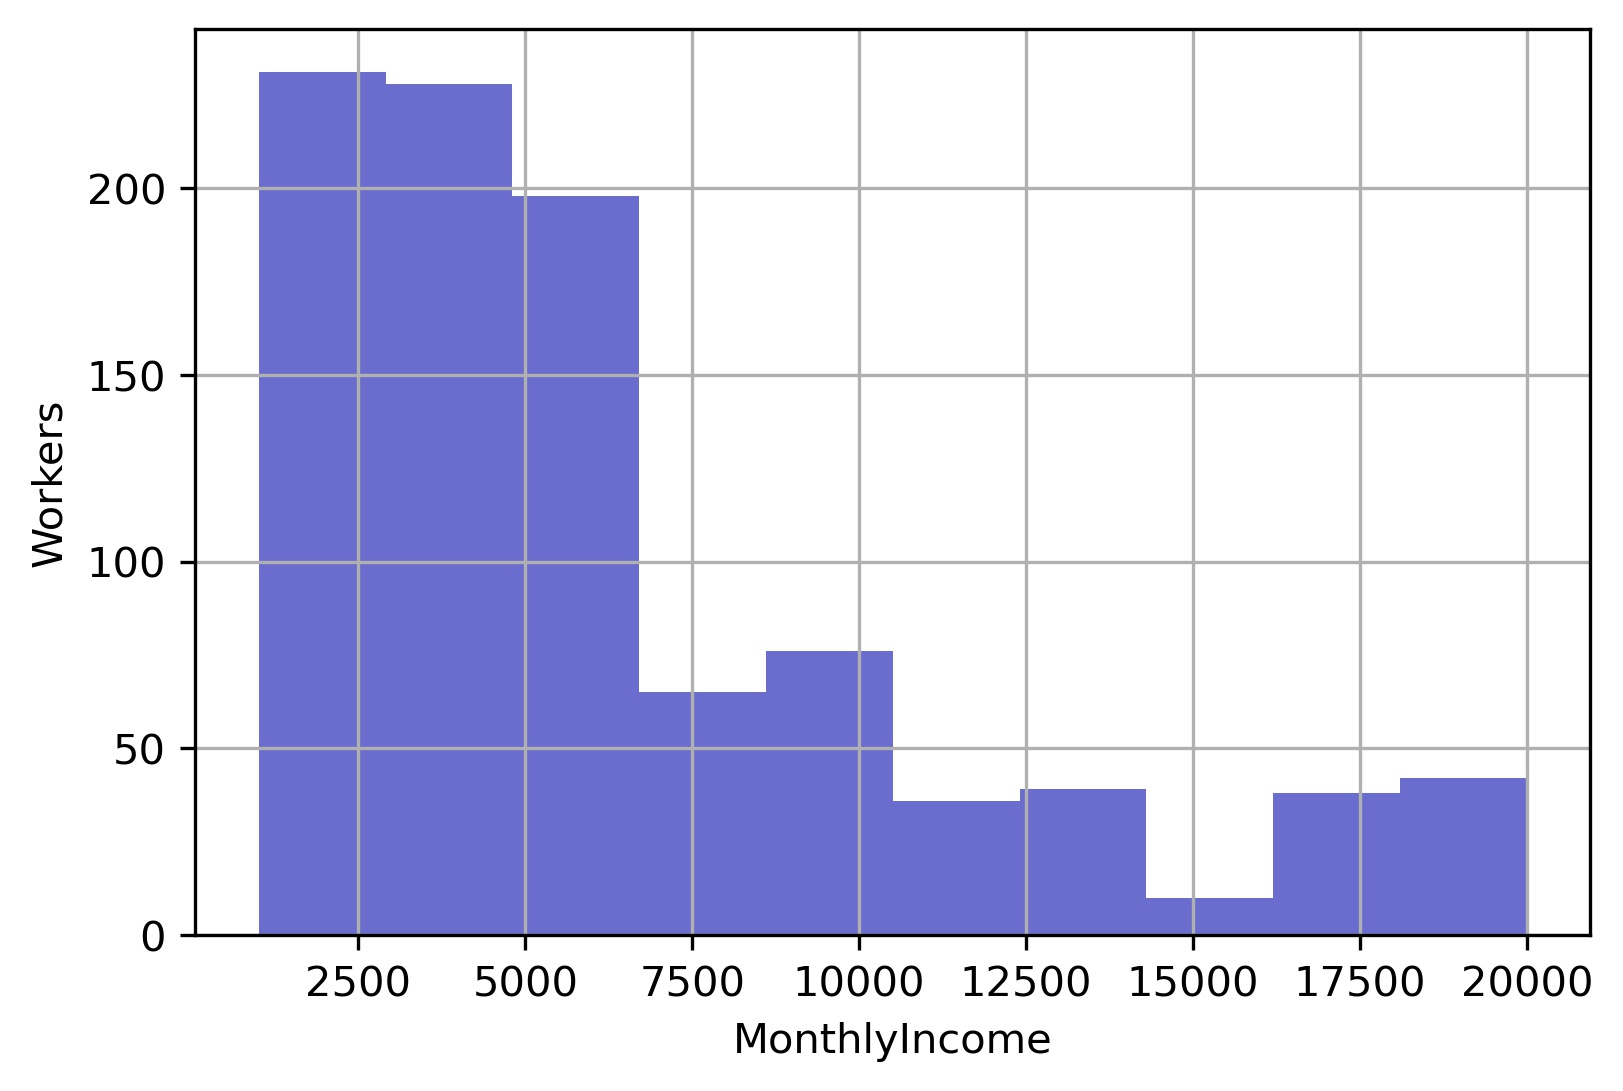
\includegraphics[width =0.45\textwidth]{Immagini/MonthlyIncome.jpeg}
		\label{DistrMonthlyIncome}
	}
	\quad
	\subfloat[]
	{
		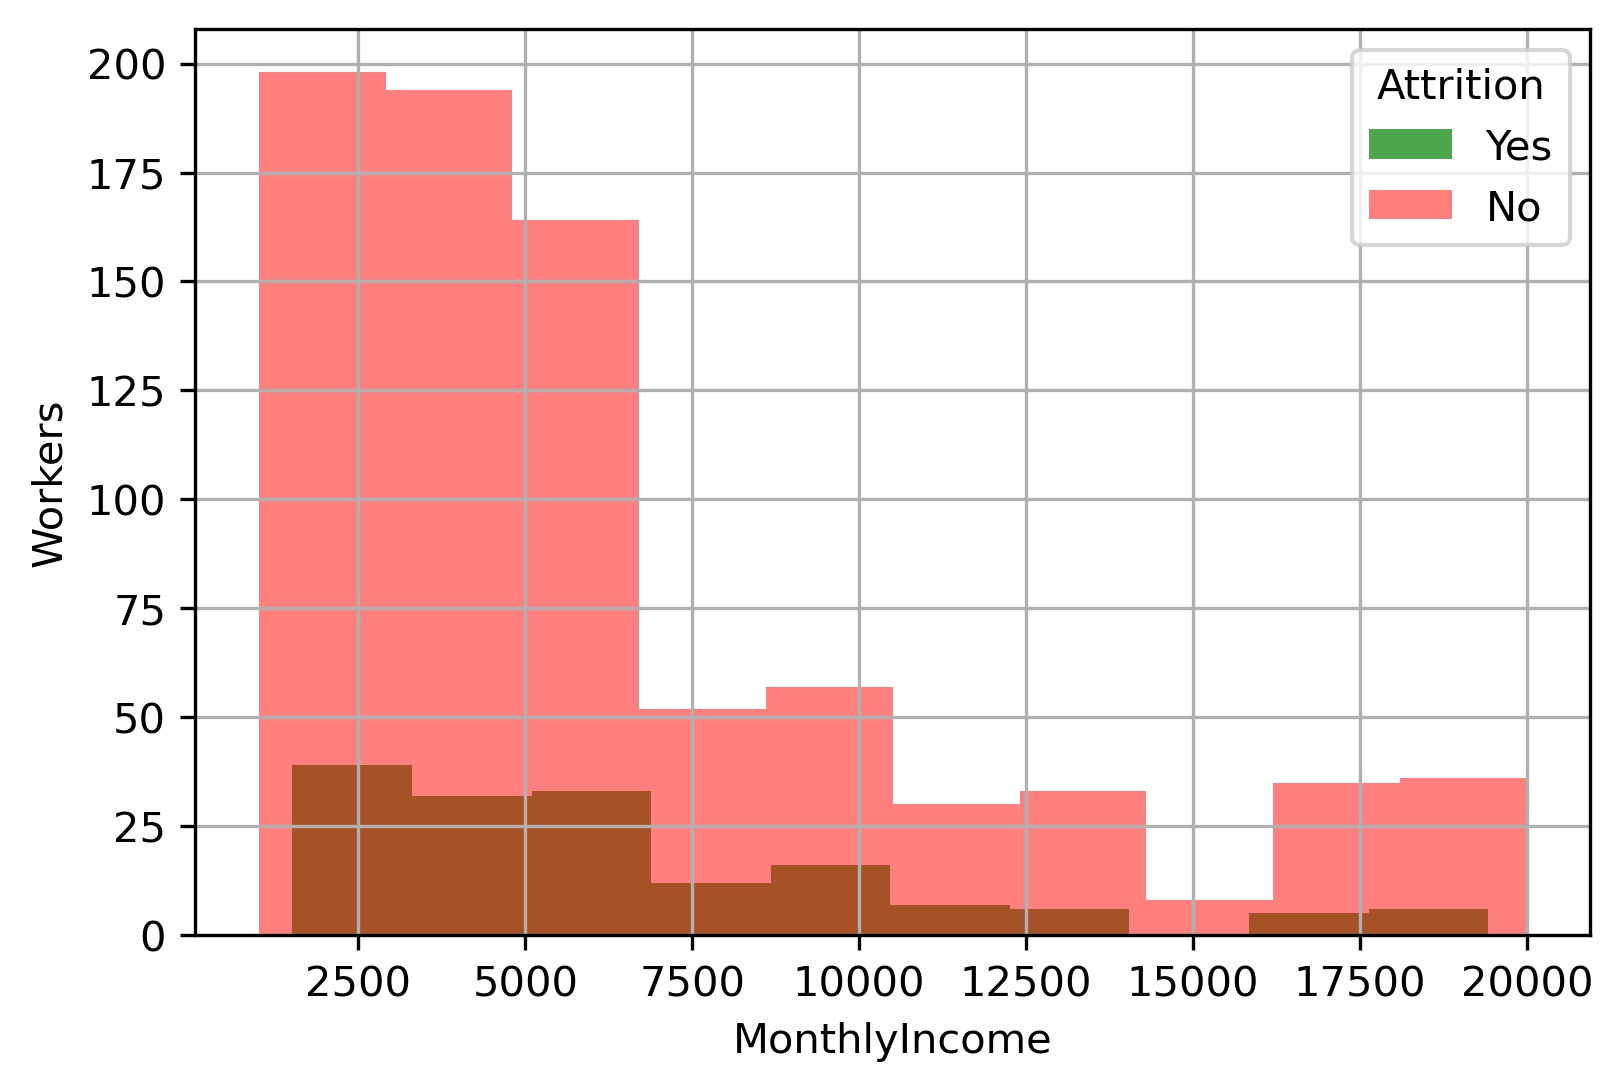
\includegraphics[width=0.45\textwidth]{Immagini/Attrition_MonthlyIncome1.jpeg}
		\label{AttrMonthlyIncome}
	}
	\caption{Distribuzione statistica dello stipendio mensile e del tasso di \textit{Attrition} in base allo stipendio}
	\label{GraficiStipendio}
\end{figure}
\noindent Come rappresentato in figura \ref{AttrMonthlyIncome}, la maggior parte delle persone che hanno deciso di lasciare il proprio posto di lavoro otteneva a fine mese uno stipendio compreso in un range basso. Tuttavia, anche in questo grafico, come in quello precedente, si nota un lieve incremento di \textit{Attrition} in corrispondenza di stipendi elevati: in questo contesto, si può ipotizzare che la crescita dei valori positivi di \textit{Attrition} sia dovuta a possibili pensionamenti.
\\\\
\textbf{\textit{YearsSinceLastPromotion}} è la \textit{\textit{feature}} che descrive gli anni trascorsi dall'ultima promozione. Anche la sua distribuzione, come quella della \textit{\textit{feature}} precedente, è fortemente sbilanciata verso lo zero (cfr. Figura \ref{PromozioneLavoro}). È interessante notare come anche i valori dell'\textit{Attrition} sono più elevati in corrispondenza dei valori 0 e 1; ciò potrebbe significare che molti lavoratori decidono di cambiare azienda dopo il primo periodo di formazione, oppure, dopo pochi anni dall'assunzione.\\\\
\begin{figure}[H]
	\centering
	\subfloat[]
	{
		\label{PromozioneLavoro}
		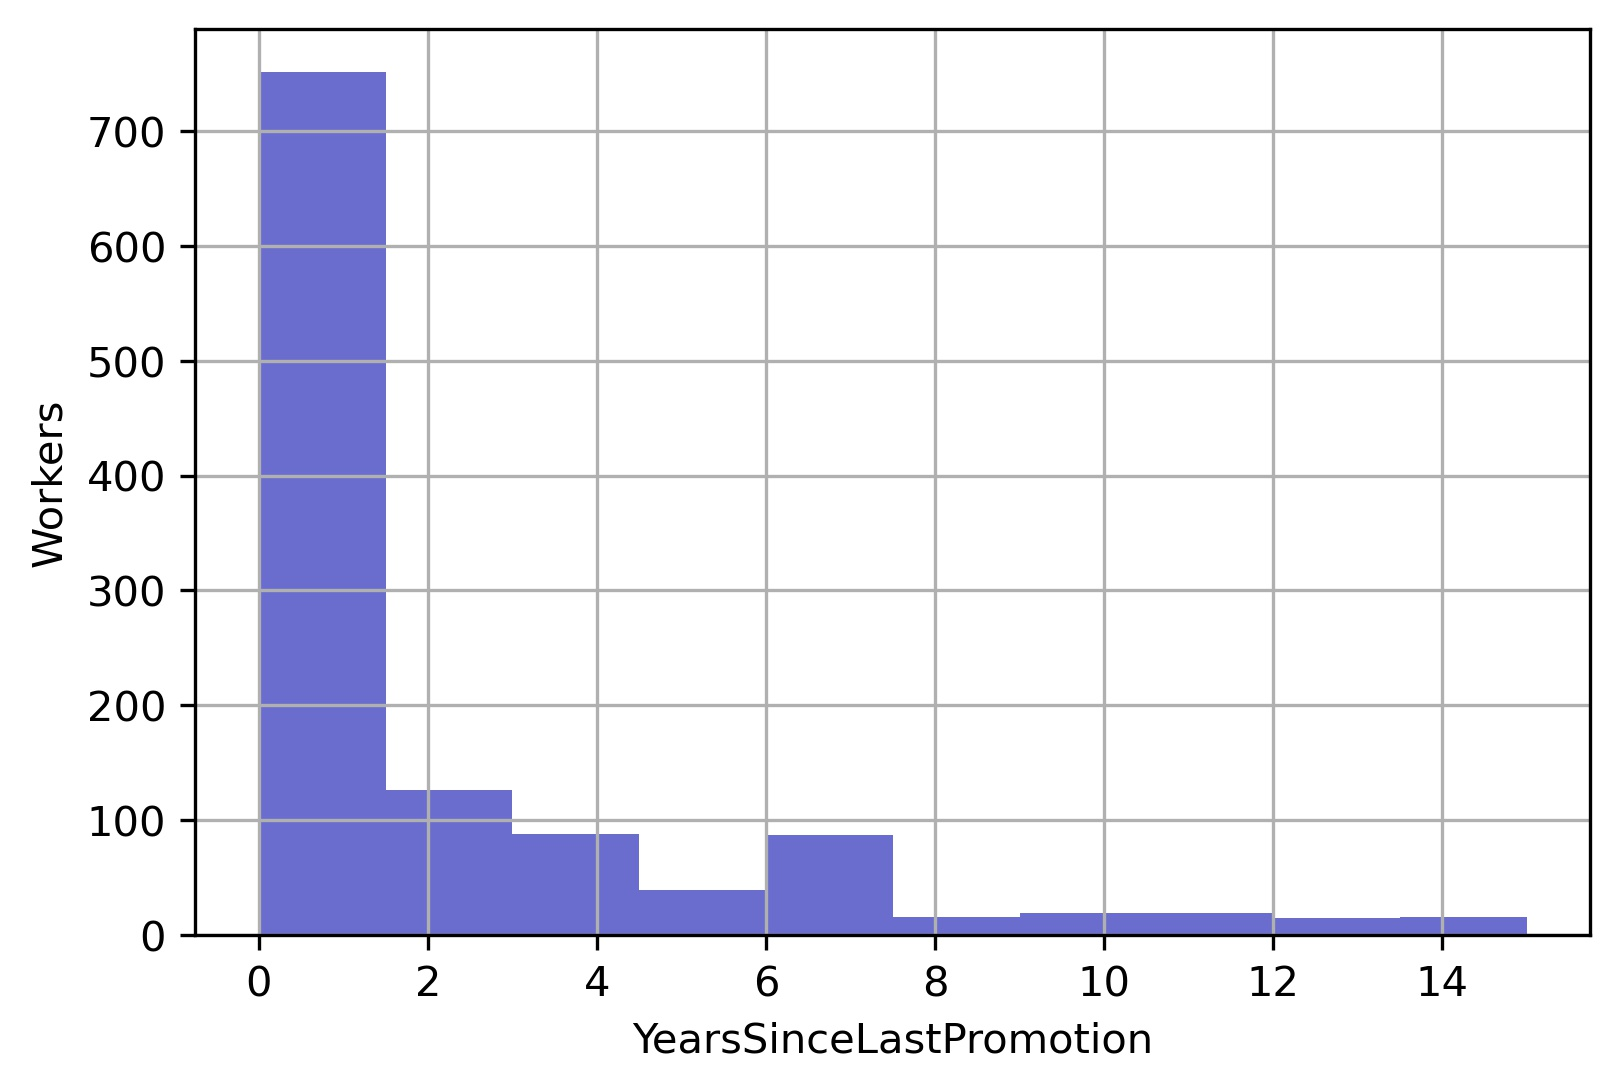
\includegraphics[width=.45\textwidth]{Immagini/YearsSinceLastPromotion.jpeg}
	}
	\quad
	\subfloat[]
	{
		\label{AttritionPromozione}
		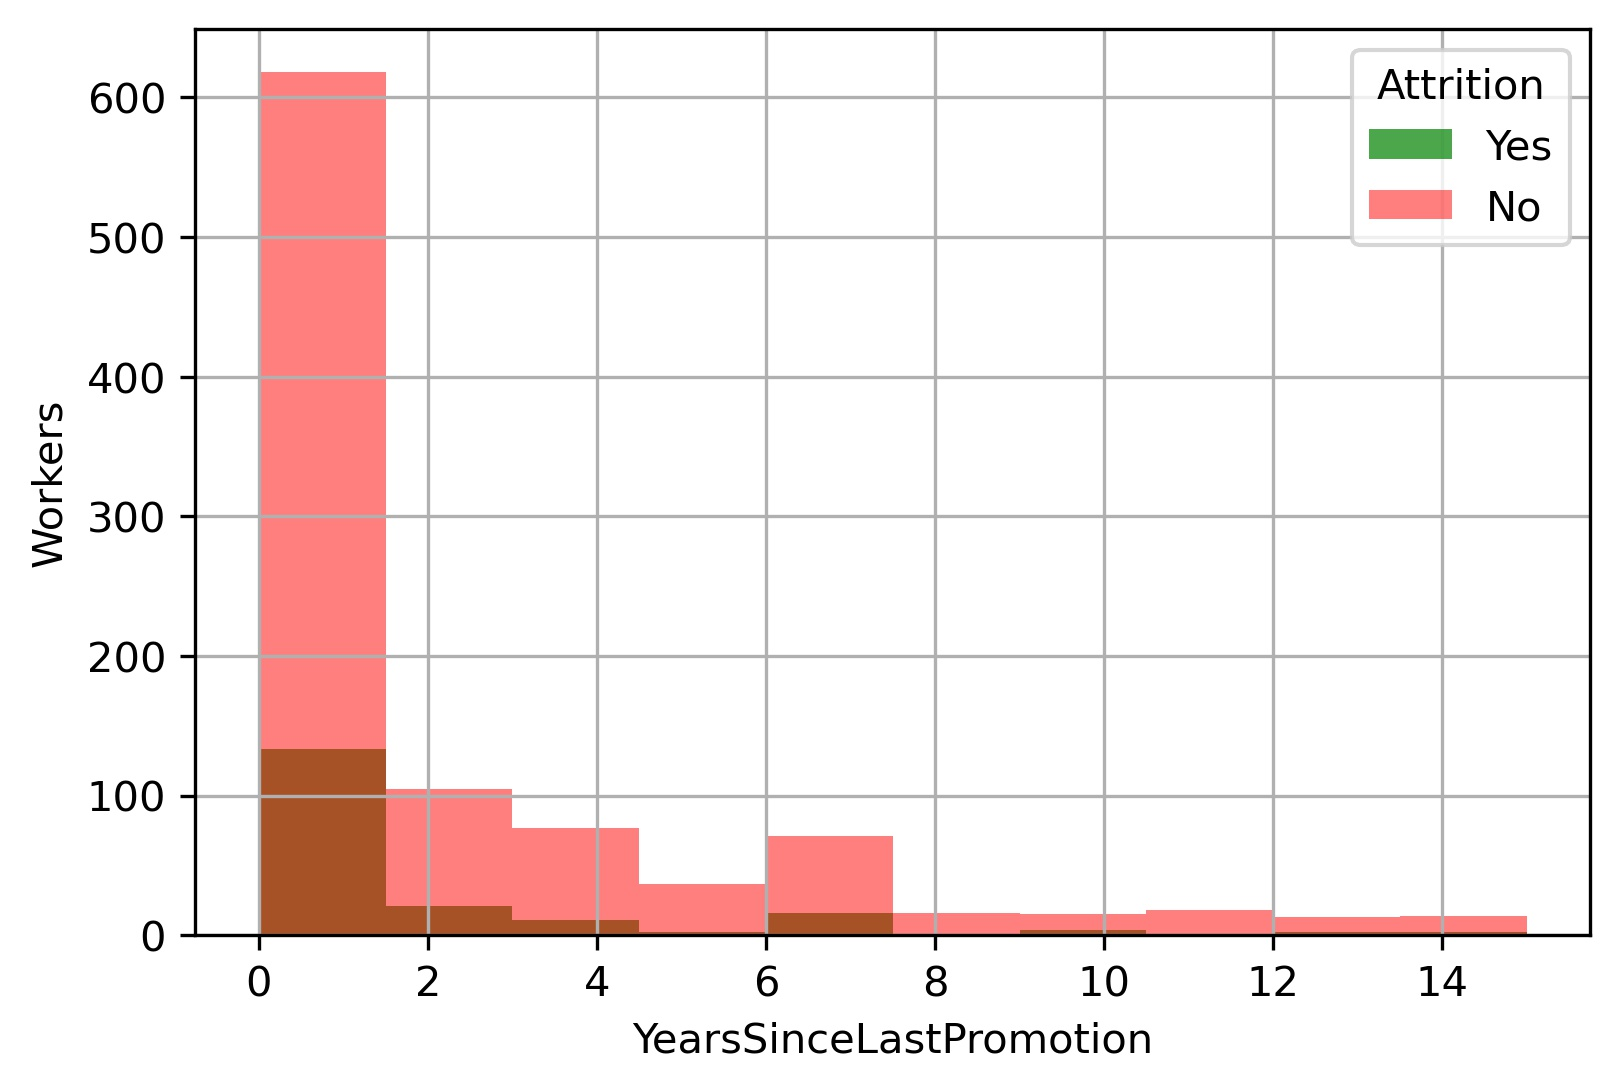
\includegraphics[width=.45\textwidth]{Immagini/Attrition_by_YearsSinceLastPromotion1.jpeg}
	}    \setlength{\belowcaptionskip}{-10pt}

	\caption{Distribuzione statistica degli anni dall'ultima promozione e del tasso di \textit{Attrition} in base allo stipendio}
	\label{GraficiPromozioneLavoro}
\end{figure}

\vspace{2em}

\begin{wrapfigure}{R}{0.50\textwidth}
    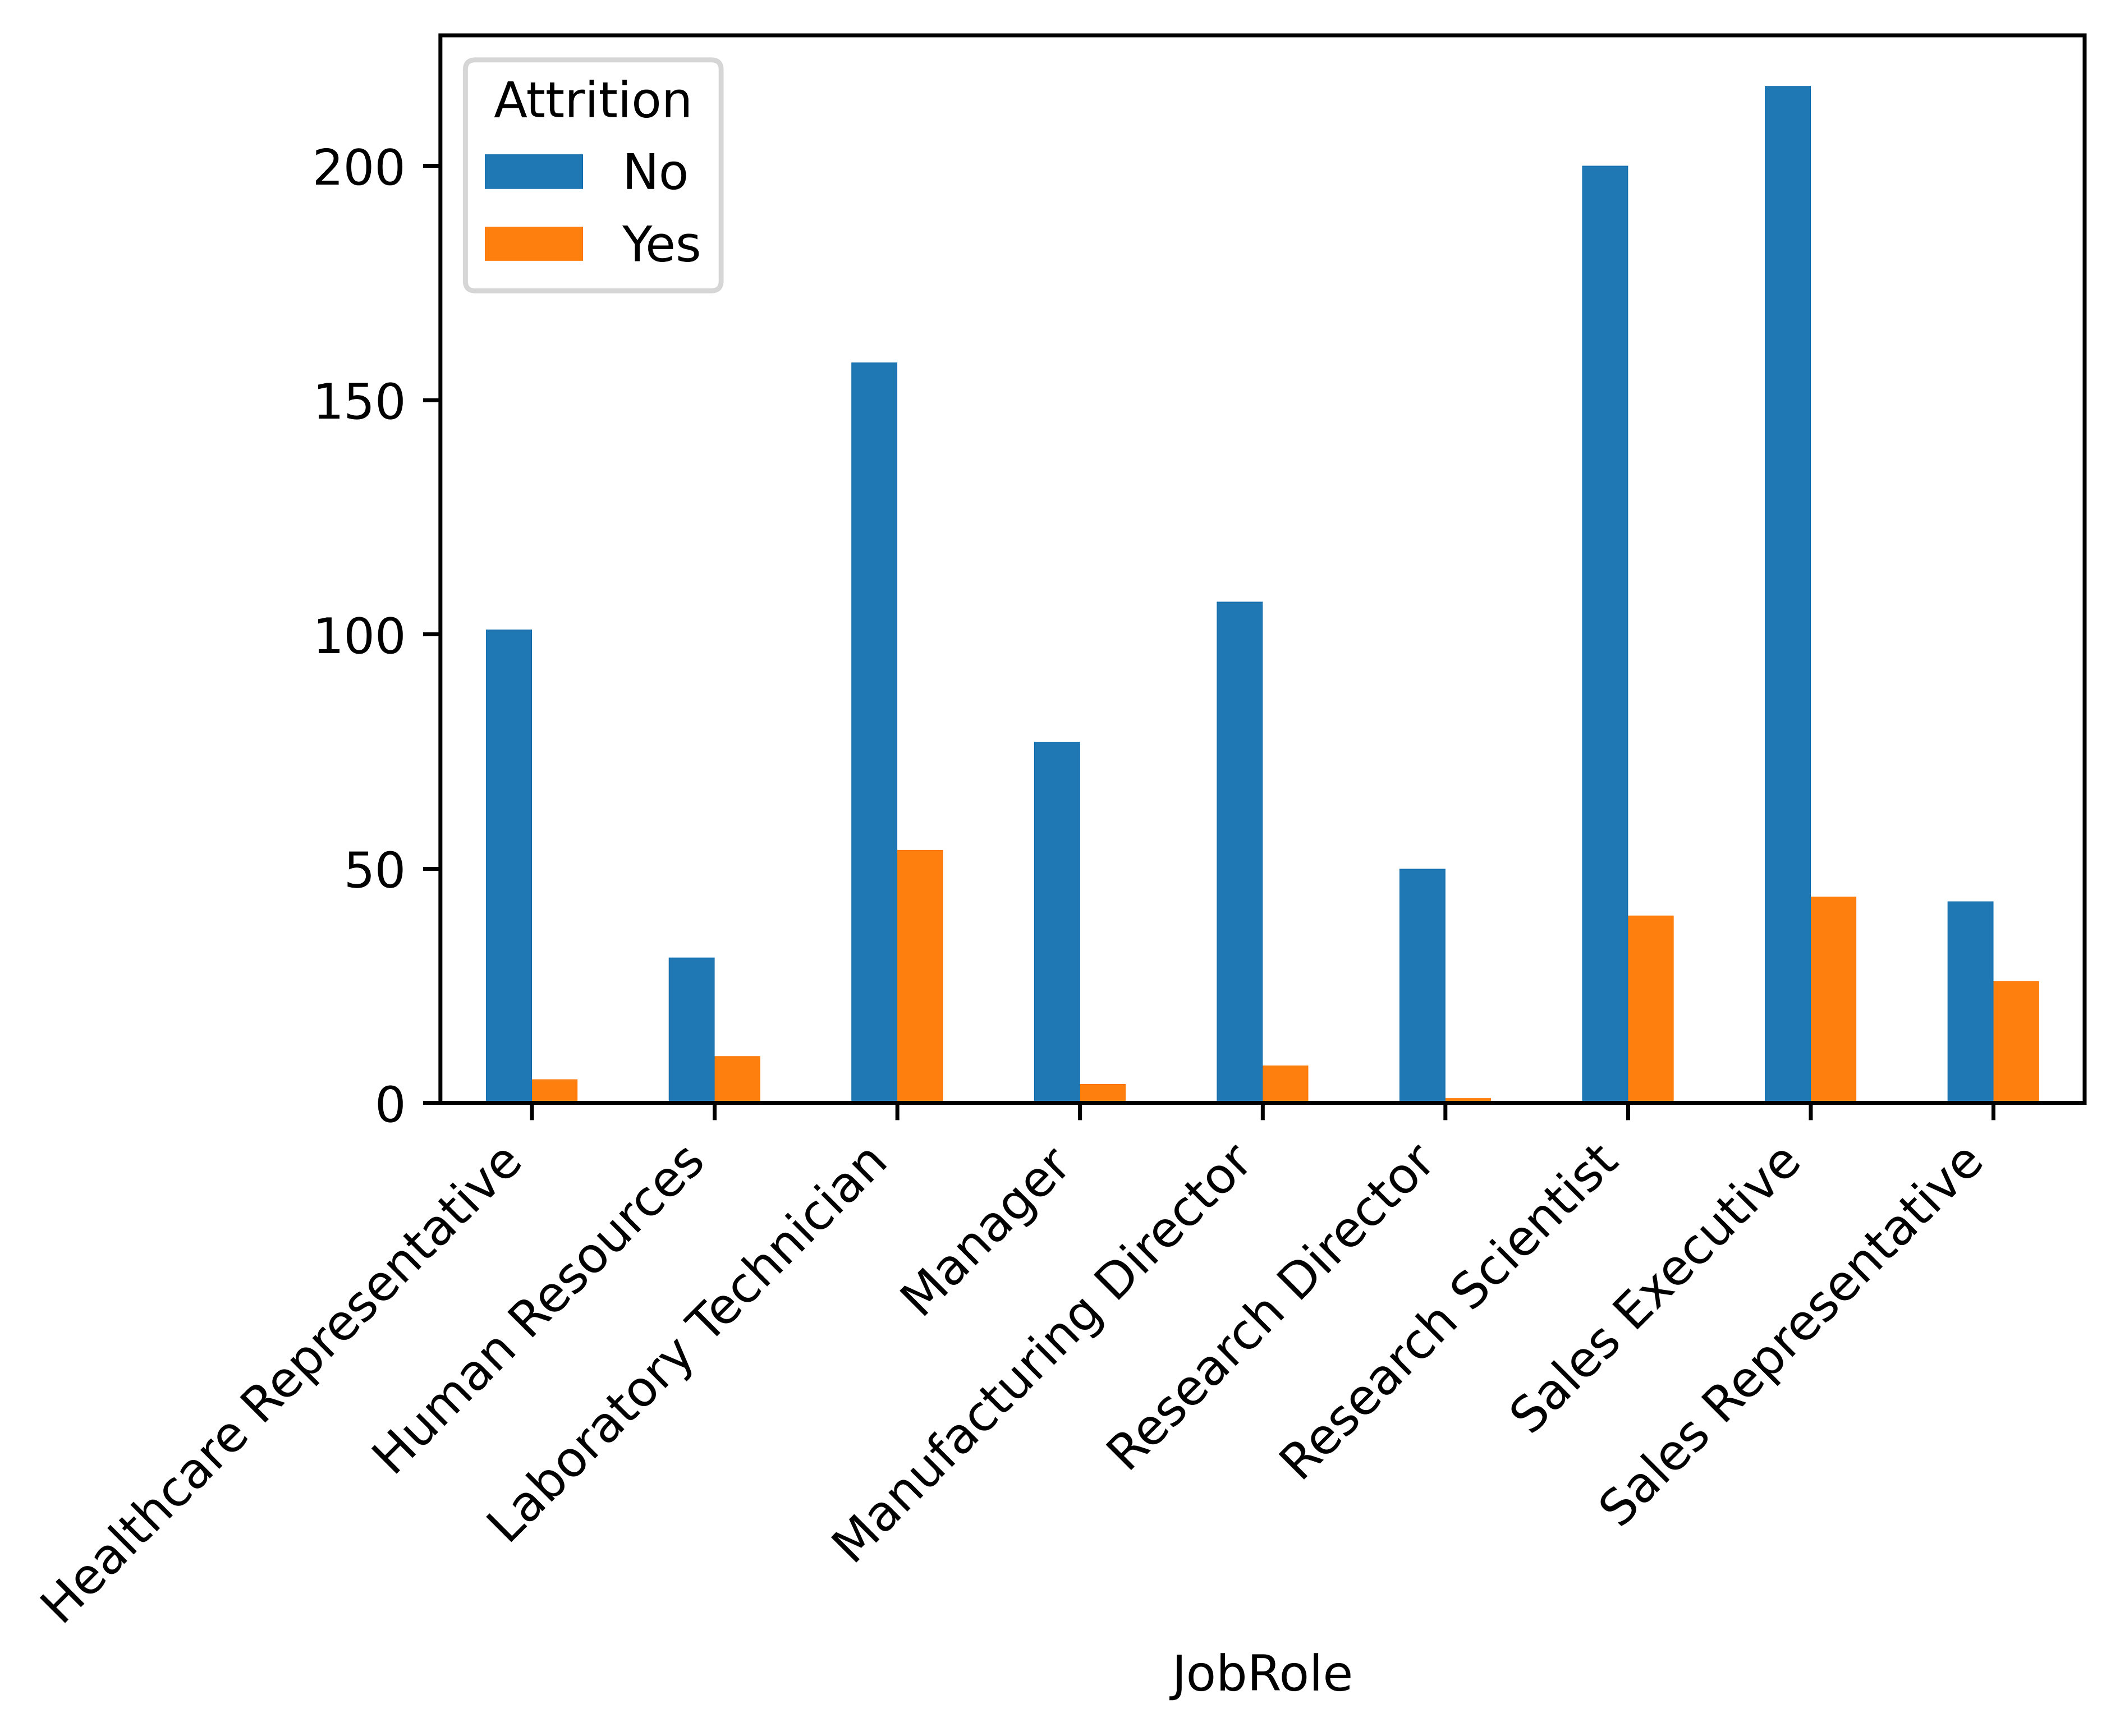
\includegraphics[width=0.49\textwidth]{Immagini/attritionRuolo.png}
    \setlength{\belowcaptionskip}{-10pt}
    \caption{Distribuzione della \textit{\textit{feature} Attrition} correlata al \textit{JobRole}}
     \clearpage
    \label{attritionJobRole}
\end{wrapfigure}

\noindent\textbf{\textit{JobRole}} è la posizione lavorativa di ciascun dipendente. Come viene evidenziato nella Figura \ref{attritionJobRole}, i lavoratori che tendono maggiormente a lasciare l'azienda sono \textit{Laboratory Technicians}, seguiti dai \textit{Research Scientists} e \textit{Sales Executives}. 
Vi sono, invece, pochissimi dipendenti che lasciano le posizioni di \textit{Manager} e \textit{Healthcare Representative} e addirittura nessuno che lascia la posizione di \textit{Research Director}.
%----ATTRITION GENDER
\\\\\textbf{\textit{Gender}} è l'attributo riguardante il sesso dei dipendenti. Dal grafico in Figura \ref{Attrition_Gender} notiamo che la quantità di persone che decidono di lasciare l'azienda è più equilibrata rispetto a quella osservata in \textit{JobRole}, sebbene in proporzione siano più gli uomini a prendere questa decisione rispetto alle donne. Abbiamo inoltre deciso di visualizzare la distribuzione del \textit{Gender} in base alla posizione lavorativa: anche in questo ambito le professioni appaiono più equamente distribuite tra i sessi (cfr. Figura \ref{JobRole_Gender}). Per le donne spiccano i valori associati a \textit{Laboratory Technician} e a \textit{Research Scientists}: in proporzione, infatti, risulta una maggior presenza di donne in questi settori rispetto agli uomini. Per i dipendenti di sesso maschile, invece, saltano all'occhio le professioni di \textit{Sales Executive} e \textit{Healthcare Representative}. \begin{figure}[H]
	\centering
	\subfloat[]
	{
		\label{Attrition_Gender}
		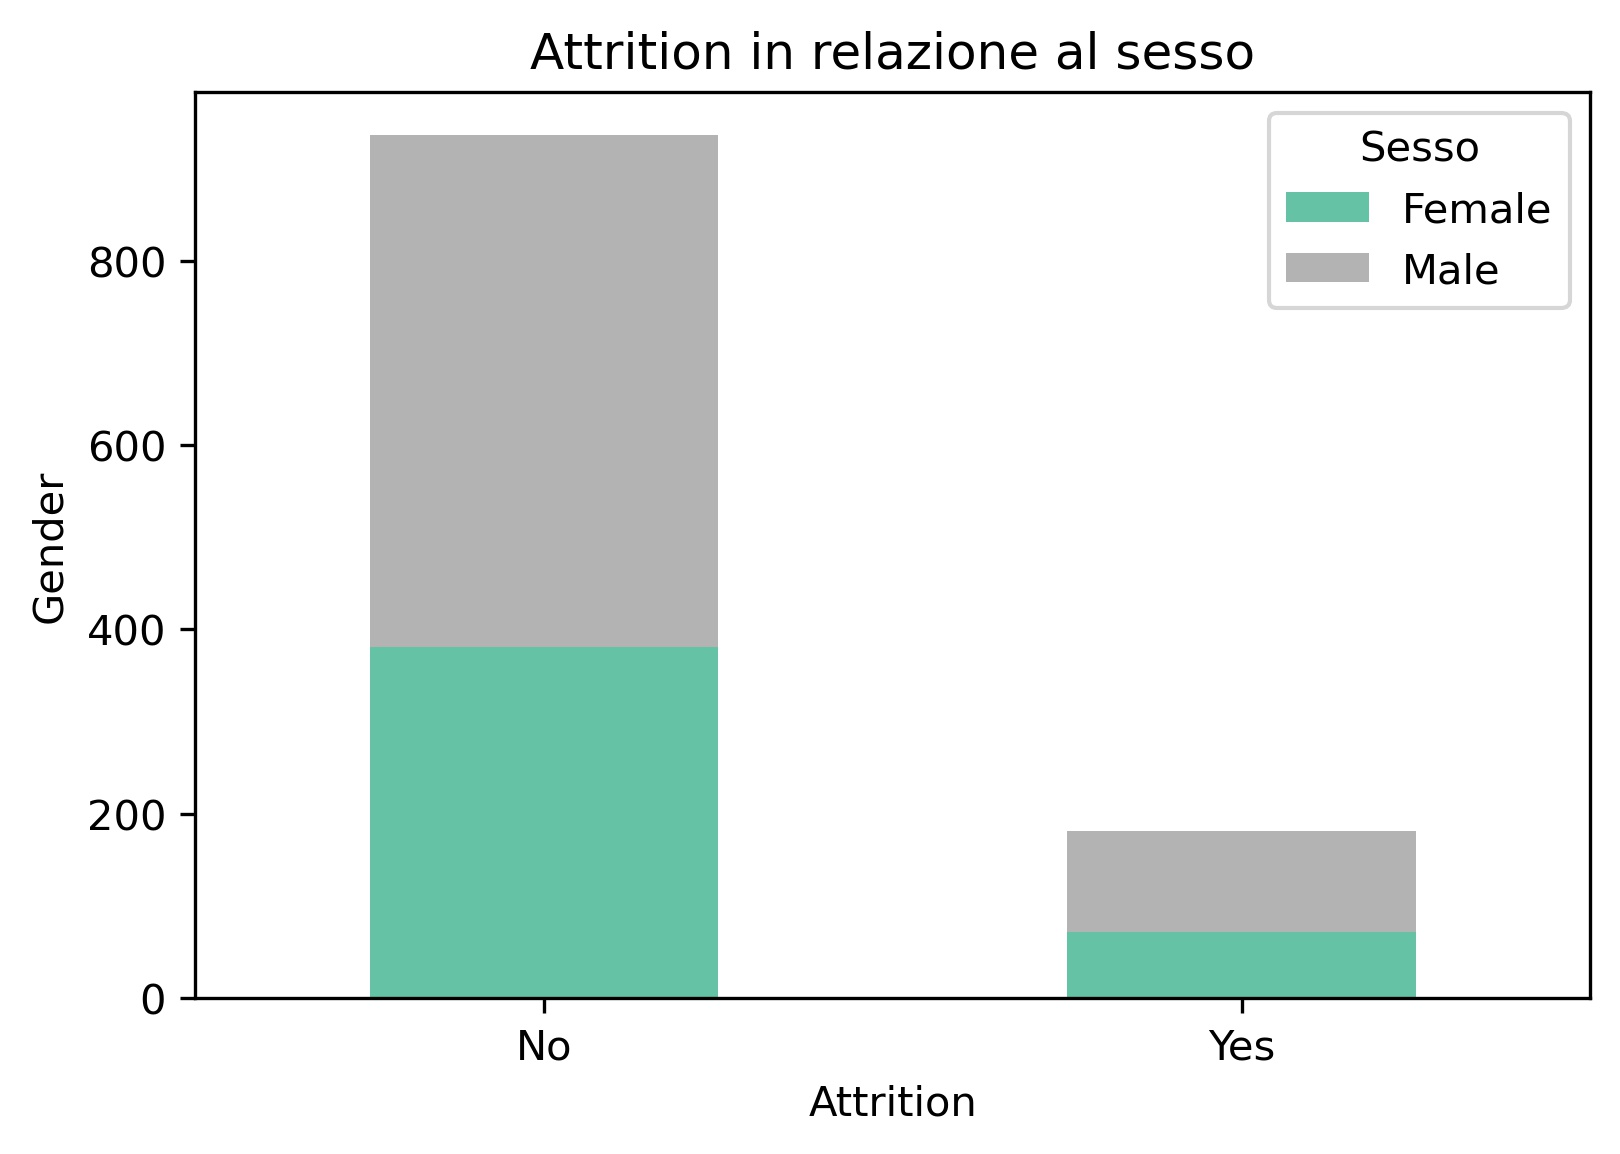
\includegraphics[width=.43\textwidth]{Immagini/Attrition_By_Gender1.jpeg}
	}
	\quad
	\subfloat[]
	{
		\label{JobRole_Gender}
		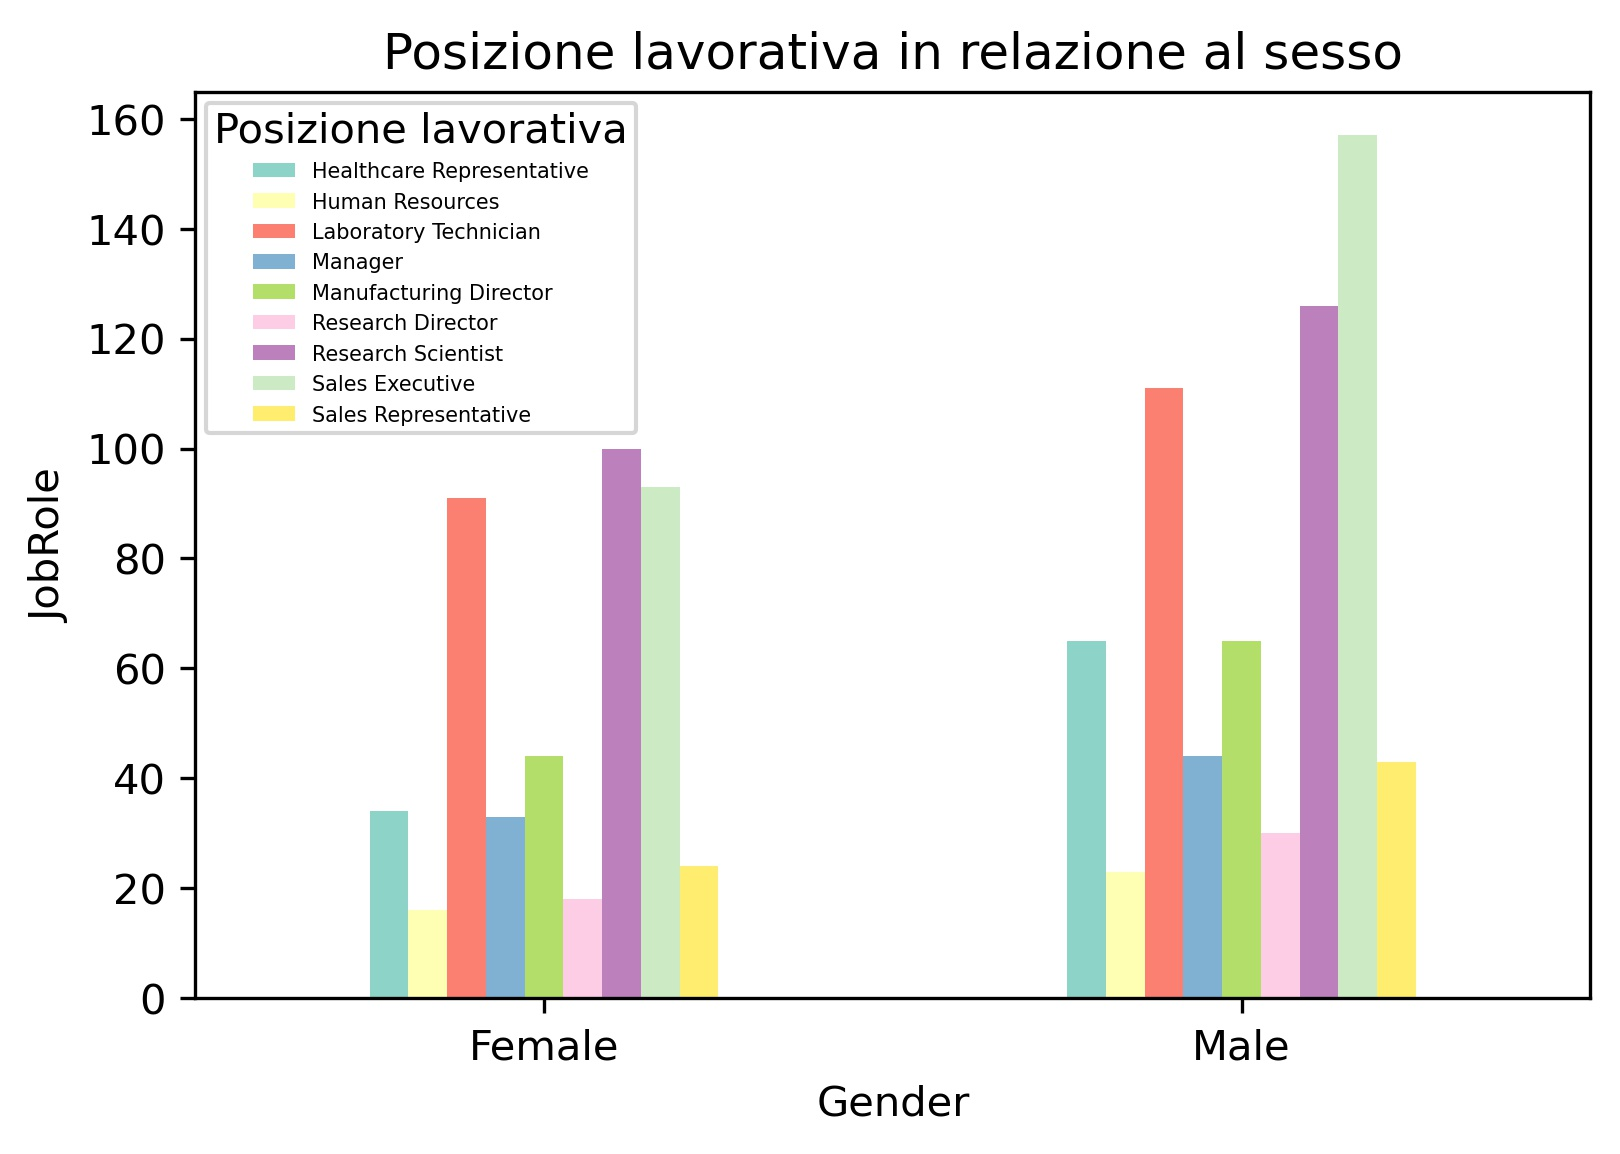
\includegraphics[width=.43\textwidth]{Immagini/JobRole_By_Gender1.jpeg}
	}
	\caption{Distribuzione dell'\textit{Attrition} in relazione al sesso dei lavoratori e distribuzione dei diversi ruoli svolti in base all'attributo \textit{Gender}}
	\label{GraficiAttrigionGenderJobRoleGender}
\end{figure}
\noindent Nella seguente tabella (Tabella \ref{statAttrNum}) abbiamo riportato le analisi statistiche applicate ai vari attributi numerici del dataset. Da questa si possono evincere alcuni valori chiave per lo studio dei dati, come ad esempio, l'età media dei lavoratori (37 anni circa) e lo stipendio mensile medio, minimo e massimo (in ordine 6566\$, 1009\$ e 19999\$). \\\\Inoltre, tenendo in considerazione le medie delle \textit{\textit{feature}} relative a \textit{Environment Satisfaction}, \textit{Job Satisfaction} e \textit{Relationship Satisfaction}, si nota che i dipendenti IBM sono  soddisfatti sia del proprio lavoro che dell'ambiente lavorativo aziendale. Infine, il livello medio di \textit{Education} tende a 3: tendenzialmente i lavoratori posseggono una laurea triennale (\textit{Bachelor's degree}).
\begin{table}[H]
\small
\centering
\resizebox{0.99\textwidth}{!}{
\begin{tabular}{|l|c|c|c|c|c|c|c|c|}
\hline
    \textbf{\textit{features}}            & \textbf{count}  & \textbf{mean}         & \textbf{std}         & \textbf{min}    & \textbf{25\%}    & \textbf{50\%}    & \textbf{75\%}     & \textbf{max}     \\ \hline\hline
Age                      & 1000.0 & 37.199000    & 9.015802    & 18.0   & 30.00   & 36.0    & 43.00    & 60.0    \\ \hline
DailyRate                & 1176.0 & 803.650510   & 406.683045  & 102.0  & 460.50  & 804.0   & 1169.00  & 1499.0  \\ \hline
DistanceFromHome         & 1176.0 & 9.210034     & 8.097024    & 1.0    & 2.00    & 7.0     & 14.00    & 29.0    \\ \hline
Education                & 1176.0 & 2.884354     & 1.016574    & 1.0    & 2.00    & 3.0     & 4.00     & 5.0     \\ \hline
EnvironmentSatisfaction  & 1176.0 & 2.715986     & 1.088876    & 1.0    & 2.00    & 3.0     & 4.00     & 4.0     \\ \hline
HourlyRate               & 1176.0 & 66.299320    & 20.266116   & 30.0   & 49.00   & 66.0    & 84.00    & 100.0   \\ \hline
JobInvolvement           & 1176.0 & 2.735544     & 0.716228    & 1.0    & 2.00    & 3.0     & 3.00     & 4.0     \\ \hline
JobLevel                 & 1176.0 & 2.021259     & 1.069686    & 1.0    & 1.00    & 2.0     & 3.00     & 5.0     \\ \hline
JobSatisfaction          & 1176.0 & 2.702381     & 1.101578    & 1.0    & 2.00    & 3.0     & 4.00     & 4.0     \\ \hline
MonthlyIncome            & 963.0  & 6565.946002  & 4710.625603 & 1009.0 & 2969.00 & 4969.0  & 8585.00  & 19999.0 \\ \hline
MonthlyRate              & 1176.0 & 14395.836735 & 7111.845106 & 2097.0 & 8227.25 & 14434.0 & 20489.25 & 26999.0 \\ \hline
NumCompaniesWorked       & 1176.0 & 2.663265     & 2.491287    & 0.0    & 1.00    & 2.0     & 4.00     & 9.0     \\ \hline
PercentSalaryHike        & 1176.0 & 15.176871    & 3.623941    & 11.0   & 12.00   & 14.0    & 18.00    & 25.0    \\ \hline
PerformanceRating        & 1038.0 & 3.152216     & 0.359403    & 3.0    & 3.00    & 3.0     & 3.00     & 4.0     \\ \hline
RelationshipSatisfaction & 1176.0 & 2.702381     & 1.092268    & 1.0    & 2.00    & 3.0     & 4.00     & 4.0     \\ \hline
StandardHours            & 606.0  & 80.000000    & 0.000000    & 80.0   & 80.00   & 80.0    & 80.00    & 80.0    \\ \hline
StockOptionLevel         & 1176.0 & 0.783163     & 0.851385    & 0.0    & 0.00    & 1.0     & 1.00     & 3.0     \\ \hline
TotalWorkingYears        & 1176.0 & 11.019558    & 7.694848    & 0.0    & 6.00    & 10.0    & 15.00    & 40.0    \\ \hline
TrainingTimesLastYear    & 943.0  & 2.827147     & 1.273120    & 0.0    & 2.00    & 3.0     & 3.00     & 6.0     \\ \hline
WorkLifeBalance          & 1176.0 & 2.755952     & 0.707984    & 1.0    & 2.00    & 3.0     & 3.00     & 4.0     \\ \hline
YearsAtCompany           & 1116.0 & 6.926523     & 6.063193    & 0.0    & 3.00    & 5.0     & 9.00     & 40.0    \\ \hline
YearsInCurrentRole       & 1176.0 & 4.188776     & 3.637405    & 0.0    & 2.00    & 3.0     & 7.00     & 18.0    \\ \hline
YearsSinceLastPromotion  & 1176.0 & 2.171769     & 3.189785    & 0.0    & 0.00    & 1.0     & 3.00     & 15.0    \\ \hline
YearsWithCurrManager     & 1176.0 & 4.107993     & 3.601097    & 0.0    & 2.00    & 3.0     & 7.00     & 17.0    \\ \hline
\end{tabular}
}    

\caption{\textit{Statistiche degli attributi numerici con totale dei valori, media, deviazione standard, valore minimo e massimo, quartili (25\%, 50\%, 75\%).}}
 \label{statAttrNum}
\end{table}
\noindent 
Passando all'analisi dei risultati in tabella \ref{StatAttrCat}, è possibile definire una migliore profilazione dei dipendenti IBM: sono prevalentemente di sesso maschile (il 56,46\% sul totale dei dipendenti), sposati, che hanno svolto studi legati alle scienze naturali o alle discipline sanitarie. All'interno dell'azienda, i dipendenti lavoravano prevalentemente come \textit{Sales Executive}, ricercatori o tecnici di laboratorio. Si può infine evidenziare come l'81,29\% non svolga viaggi di lavoro o li effettui raramente.
\begin{table}[H]
\small
\centering
\resizebox{0.99\textwidth}{!}{
\begin{tabular}{|p{3cm}|P{1.7cm}|P{2cm}|P{2.5cm}|P{2.7cm}|P{2.5cm}|}
\hline
\textbf{\textit{features}}&\textbf{Righe non vuote}& \textbf{Valori unici}& \textbf{1° valore più frequente (moda) }& \textbf{2° valore più frequente.}& \textbf{3° valore più frequente}\\
\hline
Attrition & 1176 & 2 & No (984) & Yes (192) & / \\ 
\hline
BusinessTravel & 1069 & 3 & Travel\_Rarely (764) & Travel\_Frequently (192) & Non-Travel (113)\\
\hline
Department & 1176 & 3& Research \& Development (769) & Sales (361) & Human Resources (46)\\
\hline
EducationField & 1176 & 6 & Life Sciences (489) & Medical (370) & Marketing (125) \\
\hline
Gender & 1117 &2 & Male (664) & Female (453) & / \\
\hline
JobRole & 1176 & 9 & Sales Executive (261) & Research Scientist (240) & Laboratory Technician (212) \\
\hline
MaritalStatus & 1176 & 3 & Married (542) &  Single (383) & Divorced (251) \\
\hline
Over18 & 804 & 1 & Y (804) & / & / \\
\hline
OverTime & 1176 & 2 & No (838) & Yes (338) & / \\
\hline
\end{tabular}
}
\caption{\textit{Descrizione statistica degli attributi categorici nominali con frequenza dei primi tre valori più ricorrenti.}}
\label{StatAttrCat}
\end{table}
\section{Valutazione della qualità dei dati}
\subsection{Valori mancanti}
Sono stati rilevati valori mancanti per gli attributi: \textit{Age}, \textit{BusinessTravel}, \textit{Gender}, \textit{Over18}, \textit{MonthlyIncome}, \textit{PerformanceRating}, \textit{StandardHours}, \textit{TrainingTimesLastYear} e \textit{YearsAtCompany}. \\\\
Non si è proceduto alla correzione di \textit{Over18}, \textit{StandardHours} e \textit{PerformanceRating}: i valori presenti non permettono di effettuare una stima soddisfacente delle controparti mancanti (cfr. \textit{Attributi problematici} nella Tab. \ref{TabAttributiProblematici} e, più sotto, le considerazioni su \textit{PerformanceRating}).\\\\I valori mancati di \textit{Age} e \textit{TrainingTimesLastYear} sono stati sostituiti con la media arrotondata all’intero più vicino, mentre nel caso di \textit{BusinessTravel} e \textit{Gender} con la moda. In tutti e quattro i casi, i valori sono stati calcolati tenendo come riferimento il rispettivo \textit{JobRole}, nel tentativo di offrire una stima quanto più accurata possibile. La media delle età dei lavoratori \textit{Sales Executive}, ad esempio, è 38 anni, mentre dei \textit{Research Director} 40.

\begin{table}[H]
\centering
\begin{tabular}{|l|c|l|P{3cm}|}
\hline
\multicolumn{2}{|c|}{Attributi corretti}                                           & \multicolumn{2}{c|}{Attributi problematici}                                                                                                                                                                                                         \\ \hline
\textbf{\textit{feature}} & \textbf{Valori mancanti} (\%) & \textbf{\textit{feature}}           & \textbf{Valori} \\ 
\hline
\textbf{Age} & 176 (15\%)   & \textbf{Over18}  & \textit{NaN} 372 (32\%) 
\newline \textit{Y} 804 (68\%)                                                                    \\ 
\hline
\textbf{Gender}  & 59 (5\%)                                       & \textbf{StandardHours}     & \textit{NaN} 570 (48\%)\newline \textit{80.0} 606 (52\%)                                                                                                                                    \\ \hline
\textbf{BusinessTravel}          & 107 (9\%)                                      & \textbf{PerformanceRating} & \begin{tabular}[c]{@{}l@{}}\textit{NaN} 138 (18\%)\\ \newline\textit{3.0} 808 (69\%)\\ \newline \textit{4.0} 158 (13\%)\end{tabular} \\ \hline
\end{tabular}
\caption{Valori mancanti: attributi corretti e problematici}
    \label{TabAttributiProblematici}
    \end{table}
    
\subsection{Errori nel dataset}
In \textit{MonthlyIncome} e \textit{YearsAtCompany} ai valori mancanti si accompagnano svariati errori di correttezza semantica.\\\\
Il confronto fra \textit{YearsAtCompany} e gli analoghi attributi \textit{TotalWorkingYears}, \textit{YearsInCurrentRole}, \textit{YearsSinceLastPromotion} e \textit{YearsWithCurrManager}, o con \textit{Age} e \textit{NumCompaniesWorked}, mostra in molti casi valori contraddittori\footnote{Ad esempio, \textit{TotalWorkingYears} dovrebbe essere sempre superiore a \textit{YearsAtCompany} e, trattandosi IBM di una compagnia statunitense, la differenza fra qualsiasi parametro riferito agli anni lavorativi e \textit{Age} non dovrebbe mai essere superiore a 14.}. \\\\ Singolarmente, \textit{YearsAtCompany} non mostra poi alcuna correlazione con \textit{Attrition}. Si è notato che rimuovendo gli \textit{outlier} si ha un lieve aumento della correlazione, che rimane tuttavia al di sotto di quella degli altri attributi. Si è quindi scelto di mantenere come solo parametro riferito agli anni \textit{YearsInCurrentRole}. Per i fini del presente \textit{paper} è infatti il più interessante, mostrando una discreta correlazione con \textit{Attrition}, e la quasi perfetta corrispondenza fra suoi i valori e quelli presenti in \textit{YearsWithCurrManager} rende plausibile supporne una buona correttezza.\\\\
Analogamente si è proceduto con \textit{MonthlyIncome}, \textit{HourlyRate},  \textit{DailyRate} e \textit{MonthlyRate}, tutti quanti contraddittori fra loro. Rimuovendo gli outlier e sostituendo i valori mancanti (con la metodologia di cui sopra), \textit{MonthlyIncome} ha mostrato una correlazione con \textit{Attrition} ed è stato l'unico attributo mantenuto. 

\subsection{Rimozione degli \textit{outlier}}
Per l’analisi di alcuni degli attributi del paragrafo precedente si è fatto ricorso alla rimozione degli \textit{outlier}, individuati con l’uso di \textit{boxplot}. Di ciascun parametro è stato poi calcolato l’\textit{IQR} e si è proceduto alla rimozione dei valori non appartenenti al \textit{range interquartile}.\\\\
La stessa operazione è stata effettuata per \textit{YearsInCurrentRole}. I (pochi) \textit{outlier} rilevati confermano ulteriormente la validità di questo attributo. Nella Fig. \ref{boxplotOutliers} gli \textit{outlier} di \textit{YearsInCurrentRole} a confronto con quelli di \textit{YearsAtCompany}.
\vspace{2em}
\begin{figure}[H]
    \centering
    \small
    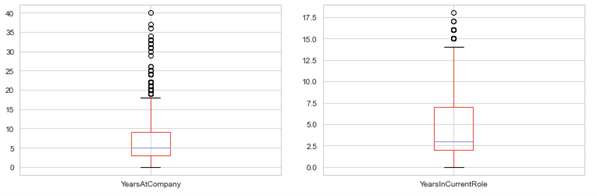
\includegraphics[width=0.68\textwidth]{Immagini/boxplot.png}
    \caption{Boxplot per \textit{YearsAtCompany} e \textit{YearsInCurrentRole}}
    \label{boxplotOutliers}
\end{figure}
\subsection{Creazione di attributi}
Per agevolare l’analisi del dataset, sono stati creati due nuovi attributi in luogo di altri già esistenti.
\begin{itemize}
\itemsep0em
    \item \textit{\textbf{GeneralEmployeeSatisfaction}}: include la media approssimata all’intero più vicino dei valori riguardanti la soddisfazione del dipendente: \textit{EnvironmentSatisfaction}, \textit{JobSatisfaction}, \textit{RelationshipSatisfaction};
    \item \textbf{\textit{CompanyInvolvement}}: include la media approssimata all’intero più vicino dei valori degli attributi indici del coinvolgimento del dipendente con le dinamiche aziendali: \textit{StockOptionLevel} e \textit{JobInvolvement}. Si noti che il primo parametro era in scala 0-3, il secondo 1-4: i valori di \textit{StockOptionLevel} sono stati dunque convertiti.
\end{itemize}

\subsection{Trasformazione dei valori}
I valori di alcuni attributi di tipo stringa sono stati convertiti in numerici\footnote{Per praticità, nel dataframe tali attributi sono stati siglati con * (es. \textit{Attrition*}).}. In particolare:
\begin{itemize}
\itemsep0em 
    \item \textit{\textbf{Attrition}}: NO $\rightarrow$ 0,  YES $\rightarrow$ 1;
    \item \textit{\textbf{Business Travel}}: Non\_Travel $\rightarrow$ 0,  Travel\_Rarely $\rightarrow$ 1,  Travel\_Frequently $\rightarrow$ 2.
    \item \textit{\textbf{Department}}: Human Resources $\rightarrow$ 0,  Research \& Development  $\rightarrow$ 1, Sales $\rightarrow$ 2;
    \item \textit{\textbf{EducationField}}: Human Resources $\rightarrow$ 0, Life Sciences $\rightarrow$ 1, Marketing $\rightarrow$ 2, Medical $\rightarrow$ 3, Other $\rightarrow$ 4, Technical Degree $\rightarrow$ 5;
    \item \textbf{\textit{Gender}}: Female $\rightarrow$ 0, Male $\rightarrow$ 1; 
    \item \textit{\textbf{JobRole}}: Healtcare Rappresentative $\rightarrow$ 0, Human Resources $\rightarrow$ 1, Laboratory Technician $\rightarrow$ 2, Manager $\rightarrow$ 3, Manufacturing Director $\rightarrow$ 4, Research Director $\rightarrow$ 5, Research Scientist $\rightarrow$ 6, Sales Executive $\rightarrow$ 7, Sales Rappresentative $\rightarrow$ 8;
    \item \textit{\textbf{MaritalStatus}}: Divorced $\rightarrow$ 0, Married $\rightarrow$ 1, Single $\rightarrow$ 2;
    \item \textbf{\textit{OverTime}}: No $\rightarrow$ 0, Yes $\rightarrow$ 1.
\end{itemize}

\subsection{Rimozione di \textit{\textit{feature}}}
La correzione degli errori e la conversione dei sopracitati valori (in particolare dell'attributo-chiave \textit{Attrition}) permettono di computare una prima \textit{matrice di correlazione}. Da essa, possiamo notare quali siano gli attributi più importanti e quali invece non abbiano alcuna particolare relazione con \textit{Attrition}. \\\\
Alla luce dei rilevamenti finora segnalati, dal dataset sono stati eliminati i seguiti attributi, oltre a quelli già citati:
\begin{itemize}
    \itemsep0em
    \item \textit{\textbf{StandardHours}} e \textbf{\textit{Over18}}: i valori non mancanti sono identici l’un l’altro, non offrendo alcuna informazione utile. \textit{Over18} risulta inoltre ridondante con \textit{Age};
    \item \textbf{\textit{PerformanceRating}}: rispetto ai due casi precedenti, i valori mancanti sono relativamente più contenuti e a livello intuitivo il parametro sarebbe stato potenzialmente molto utile per l’analisi di \textit{Attrition}. Tuttavia, l’ampia presenta di “3” a scapito di “1” e “2” (che non hanno alcuna occorrenza) inficia gravemente i possibili utilizzi di questo parametro e, a nostro avviso, la sua generale validità. È stato pertanto scartato;
    \item \textbf{\textit{Education}}, \textit{\textbf{BusinessTravel}}, \textit{\textbf{TrainingTimesLastYear}}, \textit{\textbf{NumCompaniesWorked}}, \textit{\textbf{PercentSalaryHike}}: scarsa o nulla correlazione con \textit{Attrition};
    \item \textit{\textbf{JobRole}}: il parametro è stato utile per correggere i dati mancanti, ma per le successive analisi risulta ridondante, con la presenza del più compatto \textit{Department};
    \item	\textbf{\textit{EducationField}}: nessuna correlazione con \textit{Attrition}. Per questo parametro abbiamo verificato se l’eventuale discrasia fra \textit{EducationField} e \textit{Department} possa essere una possibile causa di \textit{Attrition}, ottenendo risposta negativa. %(cfr. Figura \ref{fig:eduField}).
\end{itemize}
%\begin{figure}[H]
%    \centering
%    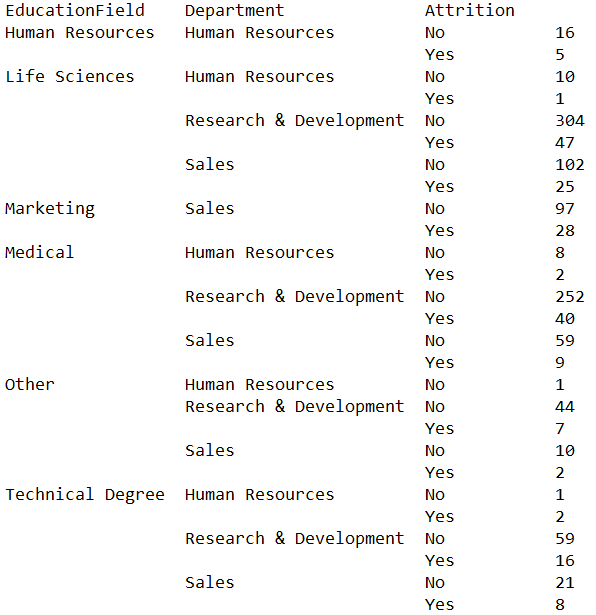
\includegraphics[scale = 0.7]{Immagini/edufield.jpg}
%    \caption{Confronto tra \textit{EducationField}, \textit{Department} e \textit{Attrition}}
%    \label{fig:eduField}
%\end{figure}
A seguito della nostra operazione di \textit{data cleaning} abbiamo ottenuto un dataset di 1029 oggetti descritti da 13 attributi. Di seguito la relativa matrice di correlazione (sono esclusi \textit{Department} e \textit{MaritalStatus}, parametri non binari originariamente categorici).
\vspace{2em}
\begin{figure}[H]
    \centering
    %\subfloat[]{{\includegraphics[scale=0.3]{Immagini/neomatrix.png} }}
    %\quad
    %\subfloat[]{{
    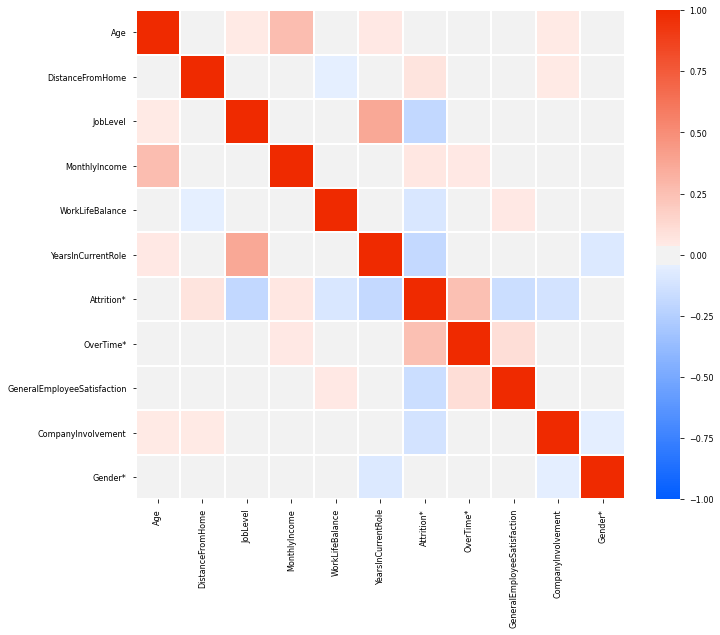
\includegraphics[scale=0.50]{Immagini/neoMatrix.png} %}}
    \caption{Matrice di correlazione dopo l'operazione di \textit{data cleaning}}
    \label{fig:MatrCorrelPostDataClean}
\end{figure}


